\chapter{Q\&A}

\section{Designing for multiple devices}

\subsection{Which size does a background image for all four resolutions need to
have?}\label{background_all_resolutions}
Since the iPad and the iPhone have different aspect ratios your
background images need to be high enough for the iPad and wide enough for the
iPhone (assuming you have a landscape game). The perfect image size is 2272px X
1536px, here is an image that explains why:

\begin{figure}[H]
		\centering
		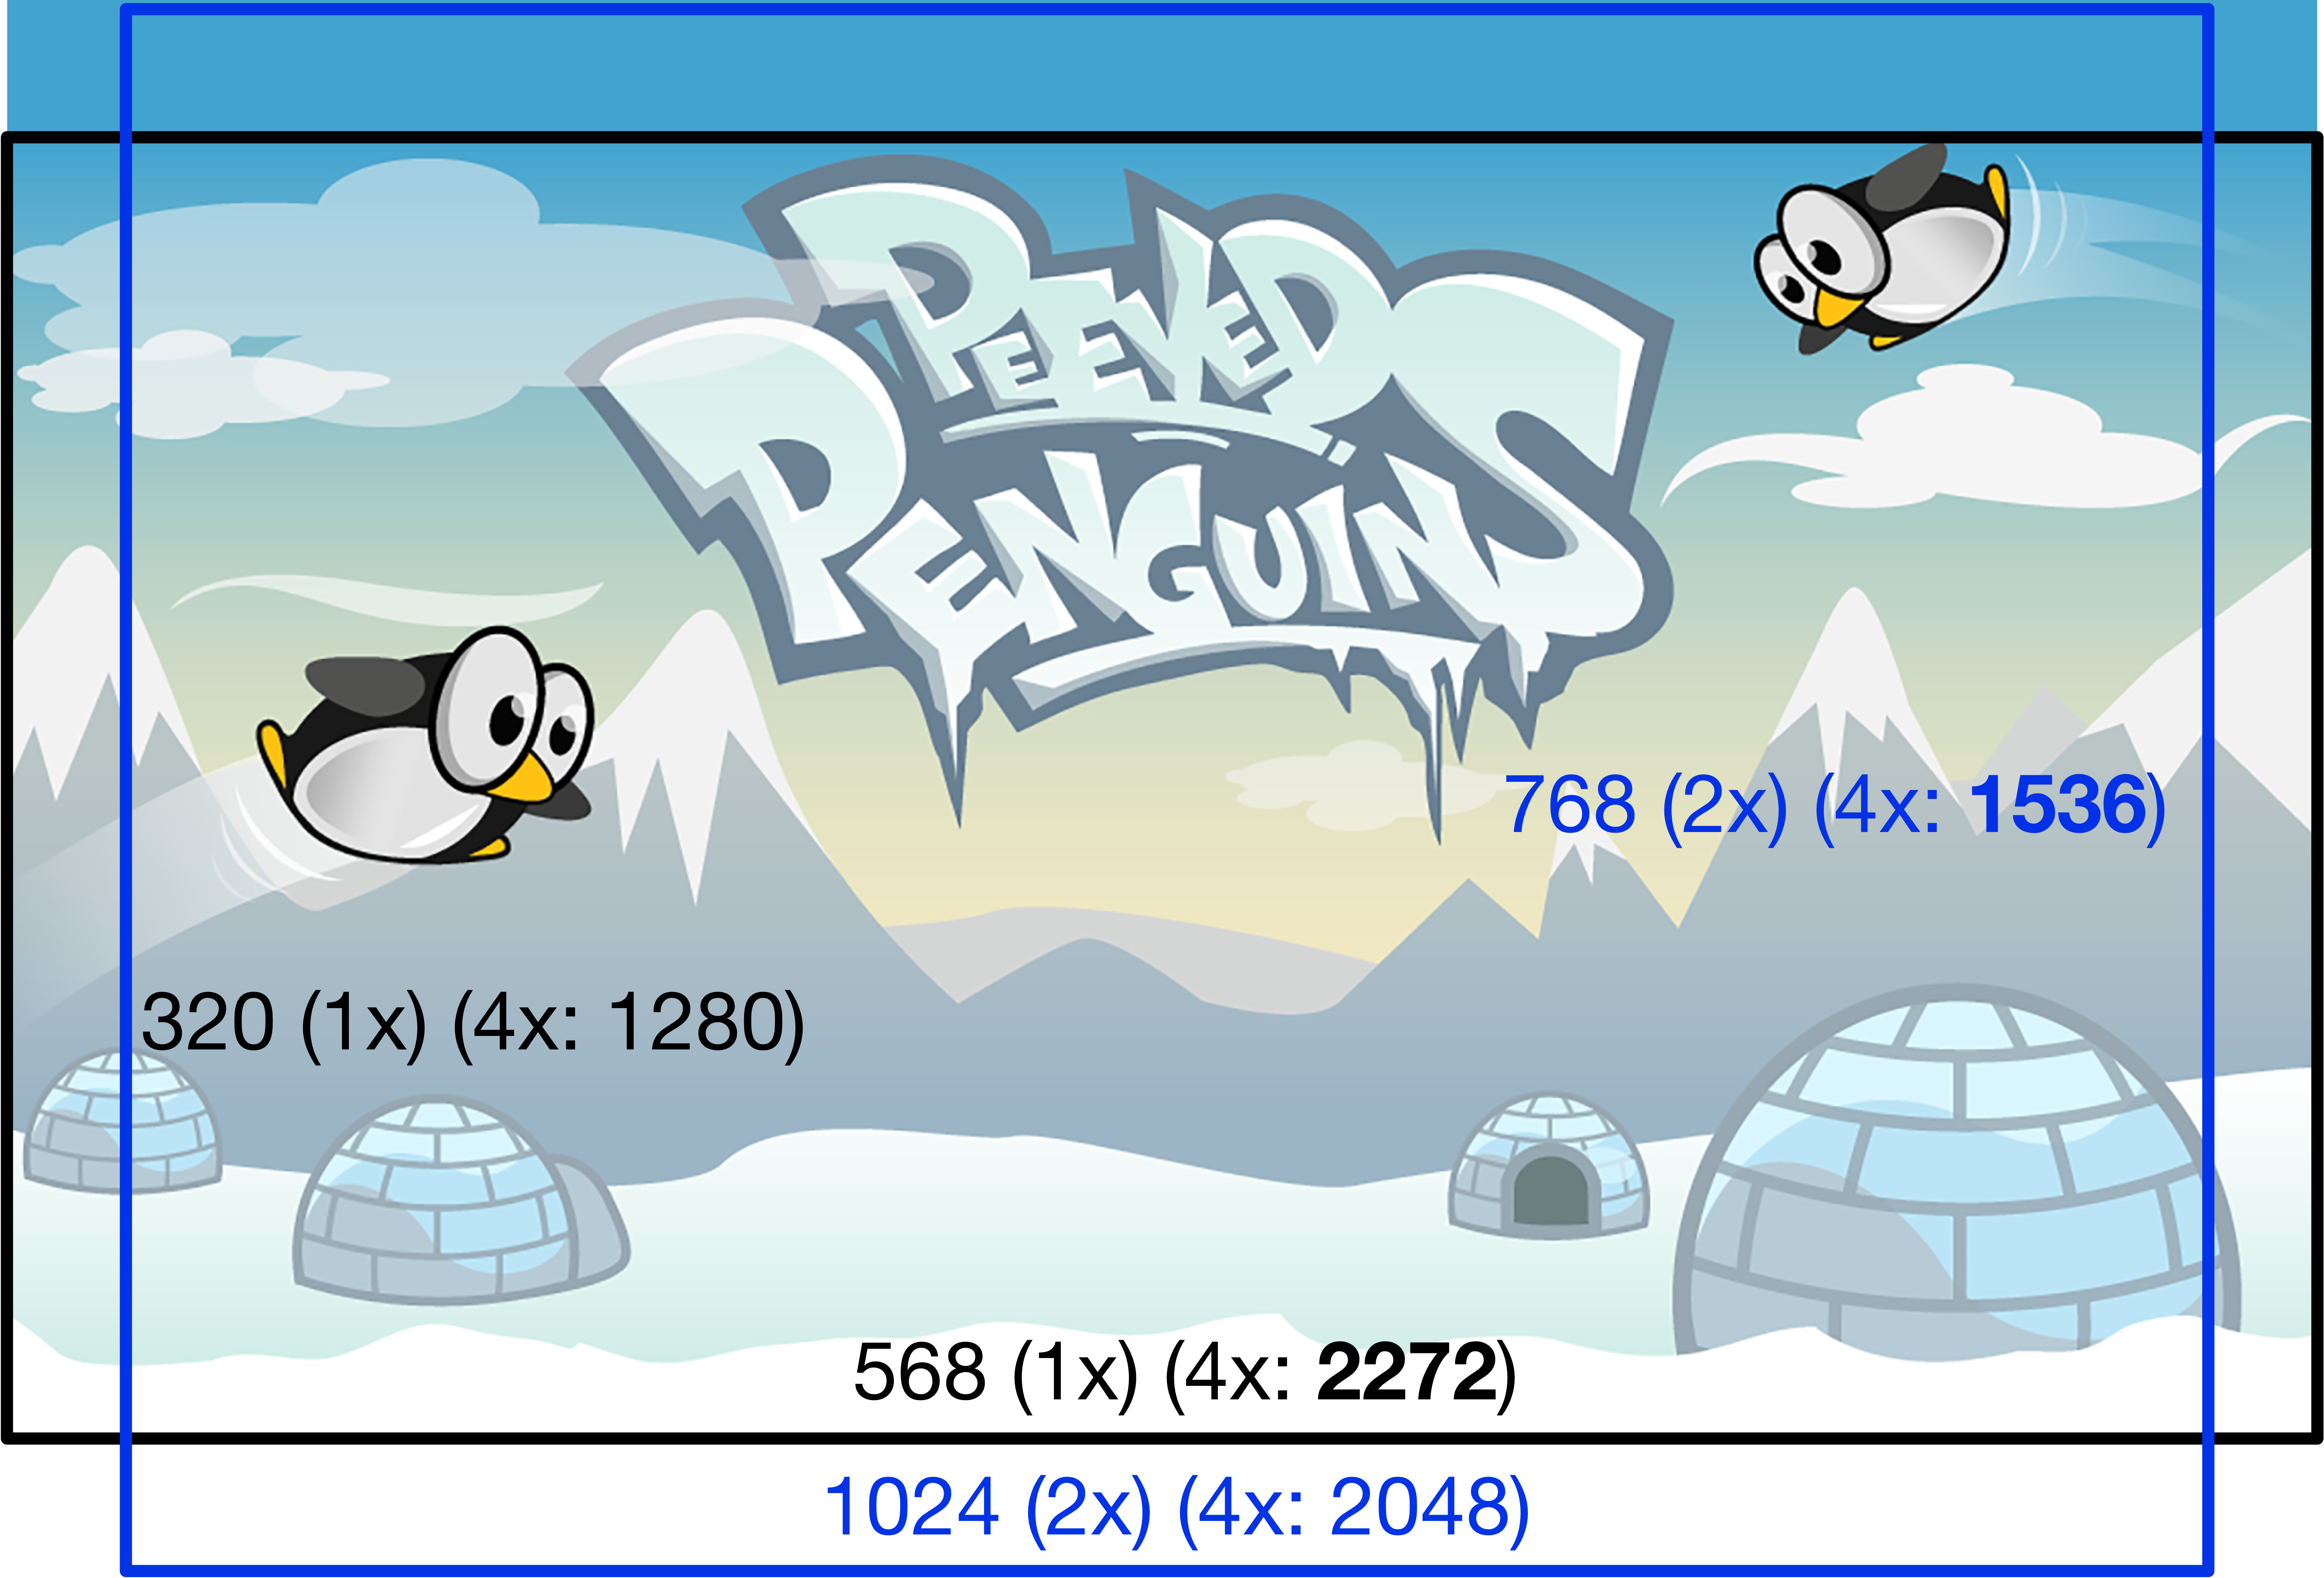
\includegraphics[height=200pt]{images/Q_A/FullScreen_AllResolutions.png}
\end{figure}

In blue you can see the outline of an iPad. An iPad has a resolution of
1024px x 768px, \SB{} uses \textit{2x} resolution for the iPad. To get the
required \textit{4x} resolution we need to multiply the value by 2, resulting in 2048px x 1536px.
In black you can see the outline of an iPhone. A 3.5-inch iPhone has a resolution
of 480px x 320px, but we want our image to also fit the 4-inch iPhone therefore
we calculate with a resolution of 568px x 320px. This is a \textit{1x}
resolution, to get to a \textit{4x} resolution we need to multiply the values by
4, resulting in a required resolution of 2272px x 1280px. You can see, the
iPhone requires a wider image, the iPad a higher one. A resolution of 2272px X
1536px satisfies both requirements. 

\section{Advance Techniques}
\subsection{Can I take a screenshot in code or even generate a level preview?}
Yes you can! \cocos{} has a awesome class called \inlinecode{CCRenderTexture}
that allows you to render a node graph into an image instead of directly to the
screen. You can use this for all kinds of features. Taking screenshots,
generating level previews or even rendering screen-in-screen!
And it is pretty simple to use, here's the outline:
\begin{lstlisting}
    CCRenderTexture *renderTexture = [CCRenderTexture renderTextureWithWidth:2048 height:self.level.contentSizeInPoints.height];
    [renderTexture beginWithClear:0 g:0 b:0 a:1.f];
    [self visit];
    [renderTexture end];
    [renderTexture saveToFile:@"Screenshot.jpeg"];
\end{lstlisting} 
